\documentclass[twoside]{book}

% Packages required by doxygen
\usepackage{fixltx2e}
\usepackage{calc}
\usepackage{doxygen}
\usepackage{graphicx}
\usepackage[utf8]{inputenc}
\usepackage{makeidx}
\usepackage{multicol}
\usepackage{multirow}
\PassOptionsToPackage{warn}{textcomp}
\usepackage{textcomp}
\usepackage[nointegrals]{wasysym}
\usepackage[table]{xcolor}

% Font selection
\usepackage[T1]{fontenc}
\usepackage{mathptmx}
\usepackage[scaled=.90]{helvet}
\usepackage{courier}
\usepackage{amssymb}
\usepackage{sectsty}
\renewcommand{\familydefault}{\sfdefault}
\allsectionsfont{%
  \fontseries{bc}\selectfont%
  \color{darkgray}%
}
\renewcommand{\DoxyLabelFont}{%
  \fontseries{bc}\selectfont%
  \color{darkgray}%
}
\newcommand{\+}{\discretionary{\mbox{\scriptsize$\hookleftarrow$}}{}{}}

% Page & text layout
\usepackage{geometry}
\geometry{%
  a4paper,%
  top=2.5cm,%
  bottom=2.5cm,%
  left=2.5cm,%
  right=2.5cm%
}
\tolerance=750
\hfuzz=15pt
\hbadness=750
\setlength{\emergencystretch}{15pt}
\setlength{\parindent}{0cm}
\setlength{\parskip}{0.2cm}
\makeatletter
\renewcommand{\paragraph}{%
  \@startsection{paragraph}{4}{0ex}{-1.0ex}{1.0ex}{%
    \normalfont\normalsize\bfseries\SS@parafont%
  }%
}
\renewcommand{\subparagraph}{%
  \@startsection{subparagraph}{5}{0ex}{-1.0ex}{1.0ex}{%
    \normalfont\normalsize\bfseries\SS@subparafont%
  }%
}
\makeatother

% Headers & footers
\usepackage{fancyhdr}
\pagestyle{fancyplain}
\fancyhead[LE]{\fancyplain{}{\bfseries\thepage}}
\fancyhead[CE]{\fancyplain{}{}}
\fancyhead[RE]{\fancyplain{}{\bfseries\leftmark}}
\fancyhead[LO]{\fancyplain{}{\bfseries\rightmark}}
\fancyhead[CO]{\fancyplain{}{}}
\fancyhead[RO]{\fancyplain{}{\bfseries\thepage}}
\fancyfoot[LE]{\fancyplain{}{}}
\fancyfoot[CE]{\fancyplain{}{}}
\fancyfoot[RE]{\fancyplain{}{\bfseries\scriptsize Generated on Thu Jan 12 2017 11\+:10\+:47 for T\+P\+Avion by Doxygen }}
\fancyfoot[LO]{\fancyplain{}{\bfseries\scriptsize Generated on Thu Jan 12 2017 11\+:10\+:47 for T\+P\+Avion by Doxygen }}
\fancyfoot[CO]{\fancyplain{}{}}
\fancyfoot[RO]{\fancyplain{}{}}
\renewcommand{\footrulewidth}{0.4pt}
\renewcommand{\chaptermark}[1]{%
  \markboth{#1}{}%
}
\renewcommand{\sectionmark}[1]{%
  \markright{\thesection\ #1}%
}

% Indices & bibliography
\usepackage{natbib}
\usepackage[titles]{tocloft}
\setcounter{tocdepth}{3}
\setcounter{secnumdepth}{5}
\makeindex

% Hyperlinks (required, but should be loaded last)
\usepackage{ifpdf}
\ifpdf
  \usepackage[pdftex,pagebackref=true]{hyperref}
\else
  \usepackage[ps2pdf,pagebackref=true]{hyperref}
\fi
\hypersetup{%
  colorlinks=true,%
  linkcolor=blue,%
  citecolor=blue,%
  unicode%
}

% Custom commands
\newcommand{\clearemptydoublepage}{%
  \newpage{\pagestyle{empty}\cleardoublepage}%
}


%===== C O N T E N T S =====

\begin{document}

% Titlepage & ToC
\hypersetup{pageanchor=false,
             bookmarks=true,
             bookmarksnumbered=true,
             pdfencoding=unicode
            }
\pagenumbering{roman}
\begin{titlepage}
\vspace*{7cm}
\begin{center}%
{\Large T\+P\+Avion }\\
\vspace*{1cm}
{\large Generated by Doxygen 1.8.7}\\
\vspace*{0.5cm}
{\small Thu Jan 12 2017 11:10:47}\\
\end{center}
\end{titlepage}
\clearemptydoublepage
\tableofcontents
\clearemptydoublepage
\pagenumbering{arabic}
\hypersetup{pageanchor=true}

%--- Begin generated contents ---
\chapter{T\+P1\+\_\+\+M\+E\+D\+E\+V}
\label{md__home_user_NetBeansProjects_TP1_MEDEV_README}
\hypertarget{md__home_user_NetBeansProjects_TP1_MEDEV_README}{}
Bataille aérienne 
\chapter{Hierarchical Index}
\section{Class Hierarchy}
This inheritance list is sorted roughly, but not completely, alphabetically\+:\begin{DoxyCompactList}
\item \contentsline{section}{Addition}{\pageref{classAddition}}{}
\item \contentsline{section}{Avion}{\pageref{classAvion}}{}
\begin{DoxyCompactList}
\item \contentsline{section}{Ennemi}{\pageref{classEnnemi}}{}
\item \contentsline{section}{Joueur}{\pageref{classJoueur}}{}
\end{DoxyCompactList}
\item \contentsline{section}{Cube}{\pageref{classCube}}{}
\item Test\begin{DoxyCompactList}
\item \contentsline{section}{Addition\+Test}{\pageref{classAdditionTest}}{}
\end{DoxyCompactList}
\end{DoxyCompactList}

\chapter{Class Index}
\section{Class List}
Here are the classes, structs, unions and interfaces with brief descriptions\+:\begin{DoxyCompactList}
\item\contentsline{section}{\hyperlink{classAddition}{Addition} }{\pageref{classAddition}}{}
\item\contentsline{section}{\hyperlink{classAdditionTest}{Addition\+Test} }{\pageref{classAdditionTest}}{}
\item\contentsline{section}{\hyperlink{classAvion}{Avion} }{\pageref{classAvion}}{}
\item\contentsline{section}{\hyperlink{classCube}{Cube} }{\pageref{classCube}}{}
\item\contentsline{section}{\hyperlink{classEnnemi}{Ennemi} }{\pageref{classEnnemi}}{}
\item\contentsline{section}{\hyperlink{classJoueur}{Joueur} }{\pageref{classJoueur}}{}
\end{DoxyCompactList}

\chapter{Class Documentation}
\hypertarget{classAddition}{\section{Addition Class Reference}
\label{classAddition}\index{Addition@{Addition}}
}
\subsection*{Static Public Member Functions}
\begin{DoxyCompactItemize}
\item 
\hypertarget{classAddition_a15d3907d8c9e9d150f89e6be205f3208}{static int {\bfseries two\+Values} (const int x, const int y)}\label{classAddition_a15d3907d8c9e9d150f89e6be205f3208}

\end{DoxyCompactItemize}


The documentation for this class was generated from the following file\+:\begin{DoxyCompactItemize}
\item 
/home/user/\+Net\+Beans\+Projects/\+T\+P1\+\_\+\+M\+E\+D\+E\+V/\+Testing/src/main.\+cpp\end{DoxyCompactItemize}

\hypertarget{classAdditionTest}{\section{Addition\+Test Class Reference}
\label{classAdditionTest}\index{Addition\+Test@{Addition\+Test}}
}


Inheritance diagram for Addition\+Test\+:
\nopagebreak
\begin{figure}[H]
\begin{center}
\leavevmode
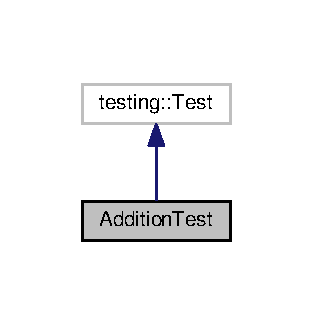
\includegraphics[width=150pt]{classAdditionTest__inherit__graph}
\end{center}
\end{figure}


Collaboration diagram for Addition\+Test\+:
\nopagebreak
\begin{figure}[H]
\begin{center}
\leavevmode
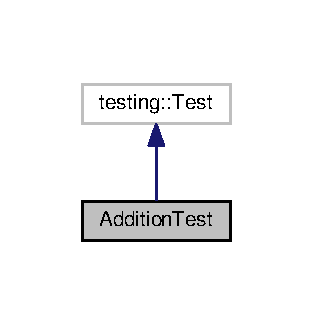
\includegraphics[width=150pt]{classAdditionTest__coll__graph}
\end{center}
\end{figure}
\subsection*{Protected Member Functions}
\begin{DoxyCompactItemize}
\item 
\hypertarget{classAdditionTest_a897f60ea7de95614df18a394384c17c4}{virtual void {\bfseries Set\+Up} ()}\label{classAdditionTest_a897f60ea7de95614df18a394384c17c4}

\item 
\hypertarget{classAdditionTest_abaf2f2b7a8583aa8db8944d79bdaf50e}{virtual void {\bfseries Tear\+Down} ()}\label{classAdditionTest_abaf2f2b7a8583aa8db8944d79bdaf50e}

\end{DoxyCompactItemize}


The documentation for this class was generated from the following file\+:\begin{DoxyCompactItemize}
\item 
/home/user/\+Net\+Beans\+Projects/\+T\+P1\+\_\+\+M\+E\+D\+E\+V/\+Testing/src/main.\+cpp\end{DoxyCompactItemize}

\hypertarget{classAvion}{\section{Avion Class Reference}
\label{classAvion}\index{Avion@{Avion}}
}


Inheritance diagram for Avion\+:
\nopagebreak
\begin{figure}[H]
\begin{center}
\leavevmode
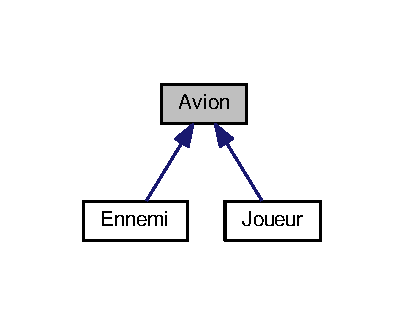
\includegraphics[width=194pt]{classAvion__inherit__graph}
\end{center}
\end{figure}
\subsection*{Public Member Functions}
\begin{DoxyCompactItemize}
\item 
\hypertarget{classAvion_aabc1d61f8cca9bb48d24858f805c4c95}{osg\+::\+Vec3f {\bfseries get\+Position} ()}\label{classAvion_aabc1d61f8cca9bb48d24858f805c4c95}

\item 
\hypertarget{classAvion_a18cfee825cfc95a63c38e9c33bbccfbe}{osg\+::\+Vec3f {\bfseries get\+Direction} ()}\label{classAvion_a18cfee825cfc95a63c38e9c33bbccfbe}

\item 
\hypertarget{classAvion_ae9d814e6736160e6732617945506ac76}{osg\+::\+Vec3f {\bfseries get\+Up} ()}\label{classAvion_ae9d814e6736160e6732617945506ac76}

\item 
\hypertarget{classAvion_a0dcfe702e314a9de909221f7646aeb04}{bool {\bfseries get\+Cooldown} ()}\label{classAvion_a0dcfe702e314a9de909221f7646aeb04}

\item 
\hypertarget{classAvion_ab697527c4adf96008244ab2656d696ba}{bool {\bfseries get\+Tir} ()}\label{classAvion_ab697527c4adf96008244ab2656d696ba}

\item 
\hypertarget{classAvion_a4499563f99a4b8c84055c43a0d7ec7b6}{float {\bfseries get\+Angle} ()}\label{classAvion_a4499563f99a4b8c84055c43a0d7ec7b6}

\item 
\hypertarget{classAvion_a069fb11c8aa32b1b957e427d66f3b92c}{float {\bfseries get\+Cap} ()}\label{classAvion_a069fb11c8aa32b1b957e427d66f3b92c}

\item 
\hypertarget{classAvion_abc7259db1069bd5703c5f239461792f3}{bool {\bfseries get\+Camp} ()}\label{classAvion_abc7259db1069bd5703c5f239461792f3}

\item 
\hypertarget{classAvion_a0791e7759e9c278a13e0987a60faabb8}{int {\bfseries get\+Id} ()}\label{classAvion_a0791e7759e9c278a13e0987a60faabb8}

\item 
\hypertarget{classAvion_ad332cfa9f8d09120011d123f98e8ee87}{void {\bfseries set\+Position} (osg\+::\+Vec3f \+\_\+position)}\label{classAvion_ad332cfa9f8d09120011d123f98e8ee87}

\item 
\hypertarget{classAvion_a64c950f24ec240aefa8343d1fda76578}{void {\bfseries set\+Direction} (osg\+::\+Vec3f \+\_\+direction)}\label{classAvion_a64c950f24ec240aefa8343d1fda76578}

\item 
\hypertarget{classAvion_af070e9bf089a987cf1ba78181145126e}{void {\bfseries set\+Up} (osg\+::\+Vec3f \+\_\+up)}\label{classAvion_af070e9bf089a987cf1ba78181145126e}

\item 
\hypertarget{classAvion_a3c088c4b5369d4a1c46fe3fc451a682f}{void {\bfseries set\+Cooldown} (bool \+\_\+cooldown)}\label{classAvion_a3c088c4b5369d4a1c46fe3fc451a682f}

\item 
\hypertarget{classAvion_a847b958c4b2c530b819196f6c0d01a99}{void {\bfseries set\+Tir} (bool \+\_\+tir)}\label{classAvion_a847b958c4b2c530b819196f6c0d01a99}

\item 
\hypertarget{classAvion_a5ebe5ab08695534b0055267b52fd3c72}{void {\bfseries set\+Angle} (float \+\_\+angle)}\label{classAvion_a5ebe5ab08695534b0055267b52fd3c72}

\item 
\hypertarget{classAvion_af022ceaeecc558ffb3774d5231953f45}{void {\bfseries set\+Cap} (float \+\_\+cap)}\label{classAvion_af022ceaeecc558ffb3774d5231953f45}

\item 
\hypertarget{classAvion_a20150470b5fc46b6fe075537ce9e11af}{void {\bfseries set\+Camp} (bool \+\_\+camp)}\label{classAvion_a20150470b5fc46b6fe075537ce9e11af}

\item 
\hypertarget{classAvion_a840877152d6d7db8184d4f5226da3320}{void {\bfseries set\+Id} (bool \+\_\+id)}\label{classAvion_a840877152d6d7db8184d4f5226da3320}

\item 
\hypertarget{classAvion_a9a757788c8f4aa550b32640953cf6654}{virtual void {\bfseries avancer} (int cube\+\_\+size)=0}\label{classAvion_a9a757788c8f4aa550b32640953cf6654}

\item 
\hypertarget{classAvion_a931f19e382481c09584e5d457e3903d4}{void {\bfseries tourner} ()}\label{classAvion_a931f19e382481c09584e5d457e3903d4}

\item 
\hypertarget{classAvion_a568ddefe4a5bbb9ffcde3cf975ae97aa}{int {\bfseries tirer} (int taillecube, std\+::vector$<$ \hyperlink{classAvion}{Avion} $\ast$ $>$ \&Liste\+Avions)}\label{classAvion_a568ddefe4a5bbb9ffcde3cf975ae97aa}

\item 
\hypertarget{classAvion_a7fdbb0c762a91c31d8bbb3be9e5c0740}{virtual void {\bfseries strategie} (std\+::vector$<$ \hyperlink{classAvion}{Avion} $\ast$ $>$ \&v)=0}\label{classAvion_a7fdbb0c762a91c31d8bbb3be9e5c0740}

\end{DoxyCompactItemize}
\subsection*{Static Public Member Functions}
\begin{DoxyCompactItemize}
\item 
\hypertarget{classAvion_a0275f22a60502f7fa484a9ad3732623c}{static void {\bfseries Detecte\+Collision} (int cube\+\_\+size, std\+::vector$<$ \hyperlink{classAvion}{Avion} $\ast$ $>$ \&avions)}\label{classAvion_a0275f22a60502f7fa484a9ad3732623c}

\end{DoxyCompactItemize}
\subsection*{Protected Attributes}
\begin{DoxyCompactItemize}
\item 
\hypertarget{classAvion_a2d3644ca8e3a7fa7d7767684656d80d4}{osg\+::\+Vec3f {\bfseries position}}\label{classAvion_a2d3644ca8e3a7fa7d7767684656d80d4}

\item 
\hypertarget{classAvion_a639ae0bce47206b55a6cbccb280196ee}{osg\+::\+Vec3f {\bfseries direction}}\label{classAvion_a639ae0bce47206b55a6cbccb280196ee}

\item 
\hypertarget{classAvion_aac1e96e696cd92cd7de6e7411cac592d}{osg\+::\+Vec3f {\bfseries up}}\label{classAvion_aac1e96e696cd92cd7de6e7411cac592d}

\item 
\hypertarget{classAvion_a39494962a6e02b4c13add30c02b5e76b}{bool {\bfseries cooldown}}\label{classAvion_a39494962a6e02b4c13add30c02b5e76b}

\item 
\hypertarget{classAvion_a0f52ac044544fe77cb8cab7df9373e82}{bool {\bfseries tir}}\label{classAvion_a0f52ac044544fe77cb8cab7df9373e82}

\item 
\hypertarget{classAvion_a982a66e25347b89477fd571792dbe9b7}{float {\bfseries angle}}\label{classAvion_a982a66e25347b89477fd571792dbe9b7}

\item 
\hypertarget{classAvion_a65c17ac385732da39a58414e3aa1d447}{float {\bfseries cap}}\label{classAvion_a65c17ac385732da39a58414e3aa1d447}

\item 
\hypertarget{classAvion_abbd0d7b37c4607e2587691e51d443433}{bool {\bfseries camp}}\label{classAvion_abbd0d7b37c4607e2587691e51d443433}

\item 
\hypertarget{classAvion_a325e2d3272cbb7b9f177b9fde05cae9a}{int {\bfseries id}}\label{classAvion_a325e2d3272cbb7b9f177b9fde05cae9a}

\end{DoxyCompactItemize}


The documentation for this class was generated from the following files\+:\begin{DoxyCompactItemize}
\item 
/home/user/\+Net\+Beans\+Projects/\+T\+P1\+\_\+\+M\+E\+D\+E\+V/include/Avion.\+h\item 
/home/user/\+Net\+Beans\+Projects/\+T\+P1\+\_\+\+M\+E\+D\+E\+V/src/Avion.\+cpp\end{DoxyCompactItemize}

\hypertarget{classCube}{\section{Cube Class Reference}
\label{classCube}\index{Cube@{Cube}}
}
\subsection*{Public Member Functions}
\begin{DoxyCompactItemize}
\item 
\hypertarget{classCube_a60e8fc89a0d4190c49dfefc901296cd1}{osg\+Viewer\+::\+Viewer $\ast$ {\bfseries get\+Viewer} ()}\label{classCube_a60e8fc89a0d4190c49dfefc901296cd1}

\item 
\hypertarget{classCube_aa6273b89c7b3d14d38f7b65b8a46e0e5}{void {\bfseries main\+Loop} ()}\label{classCube_aa6273b89c7b3d14d38f7b65b8a46e0e5}

\item 
\hypertarget{classCube_abfb120dabb6cc6f773d2fa34e31be858}{{\bfseries Cube} (int \+\_\+n)}\label{classCube_abfb120dabb6cc6f773d2fa34e31be858}

\item 
\hypertarget{classCube_a7b014d21a3c986e65bc3e56cd0b9fb60}{void {\bfseries afficher\+Cube} ()}\label{classCube_a7b014d21a3c986e65bc3e56cd0b9fb60}

\item 
\hypertarget{classCube_aac4a2abc359cc0b726599855f90b1097}{int {\bfseries get\+Size} ()}\label{classCube_aac4a2abc359cc0b726599855f90b1097}

\end{DoxyCompactItemize}
\subsection*{Public Attributes}
\begin{DoxyCompactItemize}
\item 
\hypertarget{classCube_aea71c757a46e2d0a019186e2d170c360}{bool {\bfseries fin}}\label{classCube_aea71c757a46e2d0a019186e2d170c360}

\end{DoxyCompactItemize}


The documentation for this class was generated from the following files\+:\begin{DoxyCompactItemize}
\item 
/home/user/\+Net\+Beans\+Projects/\+T\+P1\+\_\+\+M\+E\+D\+E\+V/include/Cube.\+h\item 
/home/user/\+Net\+Beans\+Projects/\+T\+P1\+\_\+\+M\+E\+D\+E\+V/src/Cube.\+cpp\end{DoxyCompactItemize}

\hypertarget{classEnnemi}{\section{Ennemi Class Reference}
\label{classEnnemi}\index{Ennemi@{Ennemi}}
}


Inheritance diagram for Ennemi\+:
\nopagebreak
\begin{figure}[H]
\begin{center}
\leavevmode
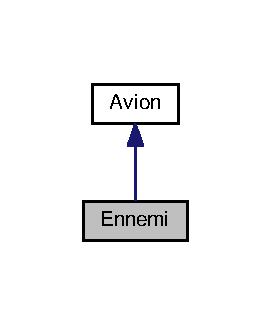
\includegraphics[width=130pt]{classEnnemi__inherit__graph}
\end{center}
\end{figure}


Collaboration diagram for Ennemi\+:
\nopagebreak
\begin{figure}[H]
\begin{center}
\leavevmode
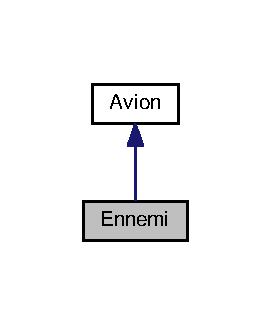
\includegraphics[width=130pt]{classEnnemi__coll__graph}
\end{center}
\end{figure}
\subsection*{Public Member Functions}
\begin{DoxyCompactItemize}
\item 
\hypertarget{classEnnemi_a8afacc285af46058850d5037cefd2d7b}{{\bfseries Ennemi} (osg\+::\+Vec3f pos, osg\+::\+Vec3f dir, int num)}\label{classEnnemi_a8afacc285af46058850d5037cefd2d7b}

\item 
\hypertarget{classEnnemi_a30f5463052d9349a4a3a561ca37b6f7a}{void {\bfseries avancer} (int cube\+\_\+size)}\label{classEnnemi_a30f5463052d9349a4a3a561ca37b6f7a}

\item 
\hypertarget{classEnnemi_a8929362ed06b114f62d7e1863303f1fc}{void {\bfseries strategie} (std\+::vector$<$ \hyperlink{classAvion}{Avion} $\ast$ $>$ \&v)}\label{classEnnemi_a8929362ed06b114f62d7e1863303f1fc}

\item 
\hypertarget{classEnnemi_a11ff402c118230c802da312bb3bc6a66}{float {\bfseries dist} (osg\+::\+Vec3f a, osg\+::\+Vec3f b)}\label{classEnnemi_a11ff402c118230c802da312bb3bc6a66}

\end{DoxyCompactItemize}
\subsection*{Additional Inherited Members}


The documentation for this class was generated from the following files\+:\begin{DoxyCompactItemize}
\item 
/home/user/\+Net\+Beans\+Projects/\+T\+P1\+\_\+\+M\+E\+D\+E\+V/include/Ennemi.\+h\item 
/home/user/\+Net\+Beans\+Projects/\+T\+P1\+\_\+\+M\+E\+D\+E\+V/src/Ennemi.\+cpp\end{DoxyCompactItemize}

\hypertarget{classJoueur}{\section{Joueur Class Reference}
\label{classJoueur}\index{Joueur@{Joueur}}
}


Inheritance diagram for Joueur\+:
\nopagebreak
\begin{figure}[H]
\begin{center}
\leavevmode
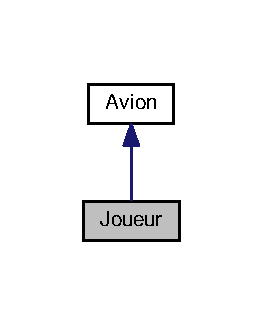
\includegraphics[width=126pt]{classJoueur__inherit__graph}
\end{center}
\end{figure}


Collaboration diagram for Joueur\+:
\nopagebreak
\begin{figure}[H]
\begin{center}
\leavevmode
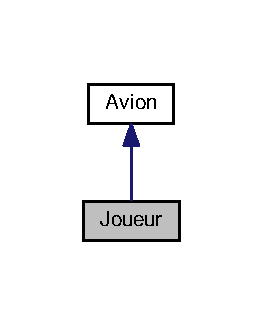
\includegraphics[width=126pt]{classJoueur__coll__graph}
\end{center}
\end{figure}
\subsection*{Public Member Functions}
\begin{DoxyCompactItemize}
\item 
\hypertarget{classJoueur_a90a46b036bb91cf837363f6c27726229}{{\bfseries Joueur} (osg\+::\+Vec3f pos, osg\+::\+Vec3f dir, int num)}\label{classJoueur_a90a46b036bb91cf837363f6c27726229}

\item 
\hypertarget{classJoueur_af72d15c1c70d15361120094d93563ba1}{void {\bfseries avancer} (int cube\+\_\+size)}\label{classJoueur_af72d15c1c70d15361120094d93563ba1}

\item 
\hypertarget{classJoueur_a7fd8856b0a69a3ba566ba9ab8c850a60}{void {\bfseries strategie} (std\+::vector$<$ \hyperlink{classAvion}{Avion} $\ast$ $>$ \&v)}\label{classJoueur_a7fd8856b0a69a3ba566ba9ab8c850a60}

\end{DoxyCompactItemize}
\subsection*{Additional Inherited Members}


The documentation for this class was generated from the following files\+:\begin{DoxyCompactItemize}
\item 
/home/user/\+Net\+Beans\+Projects/\+T\+P1\+\_\+\+M\+E\+D\+E\+V/include/Joueur.\+h\item 
/home/user/\+Net\+Beans\+Projects/\+T\+P1\+\_\+\+M\+E\+D\+E\+V/src/Joueur.\+cpp\end{DoxyCompactItemize}

%--- End generated contents ---

% Index
\newpage
\phantomsection
\addcontentsline{toc}{chapter}{Index}
\printindex

\end{document}
